\documentclass[14pt,a4paper]{article}
\usepackage[lmargin=3.81cm,rmargin=1.27cm,
vmargin=2.54cm,tmargin=2.54cm,bmargin=3.175cm]{geometry}
\usepackage{fancyhdr}
\usepackage{indentfirst}
\usepackage{graphicx}
\setlength{\parindent}{1.5cm}
\setlength{\parindent}{1.5 cm}
\setlength{\parskip}{1em}
\pagestyle{fancy}
\fancyhf{}
\rhead{Next Generation of Virtual Personal Assistants}
\rfoot{\thepage}
\lfoot{PVG’s COET COMP. DEPT. 2018-19}
\usepackage{listings}
\usepackage{color}
\definecolor{dkgreen}{rgb}{0,0.6,0}
\definecolor{gray}{rgb}{0.5,0.5,0.5}
\definecolor{mauve}{rgb}{0.58,0,0.82}
\lstset{frame=tb,
  language=Python,
  aboveskip=3mm,
  belowskip=3mm,
  showstringspaces=false,
  columns=flexible,
  basicstyle={\small\ttfamily},
  numbers=none,
  numberstyle=\tiny\color{gray},
  keywordstyle=\color{blue},
  commentstyle=\color{dkgreen},
  stringstyle=\color{mauve},
  breaklines=true,
  breakatwhitespace=true,
  tabsize=4
}

\begin{document}
\newpage
\cleardoublepage
\thispagestyle{empty}
\section{Acknowledgement}
\noindent
\par No volume of words is enough to express my gratitude towards my guide, Prof. A .M. Bhadgale, Assistant Professor in Computer Engineering Department, who has been very concerned and have aided for all the help essential for the preparation of this work. He has helped me to explore this vast topic in an organized manner and provided me with all the ideas on how to work towards a research-oriented venture.
\par  I am also thankful to Prof. M. V. Marathe, Head of Department, Computer Engineering, for the motivation and inspiration that triggered me for the seminar work.

\par
Parth Parikh  T150074247\par
(T.E. Computer Engineering)


\newpage

\section{Abstract}
\noindent
\par One of the goals of Artificial intelligence (AI) is the
realization of natural dialogue between humans and machines.
in recent years, the dialogue systems, also known as interactive
conversational systems are the fastest growing area in AI. Many
companies have used the dialogue systems technology to establish
various kinds of Virtual Personal Assistants(VPAs) based on
their applications and areas, such as Microsoft’s Cortana,
Apple’s Siri, Amazon Alexa, Google Assistant, and Facebook’s
M. However, in this proposal, we have used the multi-modal
dialogue systems which process two or more combined user input
modes, such as speech, image, video, touch, manual gestures,
gaze, and head and body movement in order to design the Next-
Generation of VPAs model. The new model of VPAs will be used
to increase the interaction between humans and the machines by
using different technologies, such as gesture recognition,
image/video recognition, speech recognition, the vast dialogue
and conversational knowledge base, and the general knowledge
base. Moreover, the new VPAs system can be used in other
different areas of applications, including education assistance,
medical assistance, robotics and vehicles, disabilities systems,
home automation, and security access control.
\newpage
\tableofcontents
\newpage
\section{Dialogflow}
\subsection{Introduction to Dialogflow}
\par Dialogflow (formerly Api.ai, Speaktoit) is a Google-owned developer of human–computer interaction technologies based on natural language conversations. Dialogflow has also created a natural language processing engine that incorporates conversation context like dialogue history, location and user preferences. It works on natural language processing and backed by Machine Learning .

\par Voice and conversational interfaces created with Dialogflow works with a wide range of devices including phones, wearables, cars, speakers and other smart devices. It supports 14+ languages including Brazilian Portuguese, Chinese, English, Dutch, French, German, Italian, Japanese, Korean, Portuguese, Russian, Spanish and Ukrainian. Dialogflow is backed by Google, incorporates Google's machine learning expertise and products such as Google Cloud Speech-to-Text and runs on Google infrastructure, which makes Dialogflow apps easily scalable to millions of users.

\par Dialogflow supports an array of services that are relevant to entertainment and hospitality industries. Dialogflow also includes an analytics tool that can measure the engagement or session metrics like usage patterns, latency issues, etc. 

\par Dialogflow uses new ways to interact with your product by building engaging voice and text-based conversational interfaces, such as voice apps and chatbots, powered by AI. Dialogflow integrations can be found on websites, mobile apps, Google Assistant, Amazon Alexa, Facebook Messenger, and other popular platforms and devices. 
The process a Dialogflow agent follows from invocation to fulfilment is similar to someone answering a question, with some liberties taken of course.

\subsection{Why use Dialogflow ?}
\begin{enumerate}
\item[•] On any platform - Dialogflow supports more than 20 platforms ranging from Google Home to Twitter.
\item[•] Across devices - Dialogflow supports all devices ranging from wearables to smart speakers and even cars.
\item[•] Around the world - Dialogflow supports more than 14 languages worldwide and more support keeps getting added.
\end{enumerate}

\subsection{Glossary of Dialogflow}
\begin{figure}[h]
\centering 
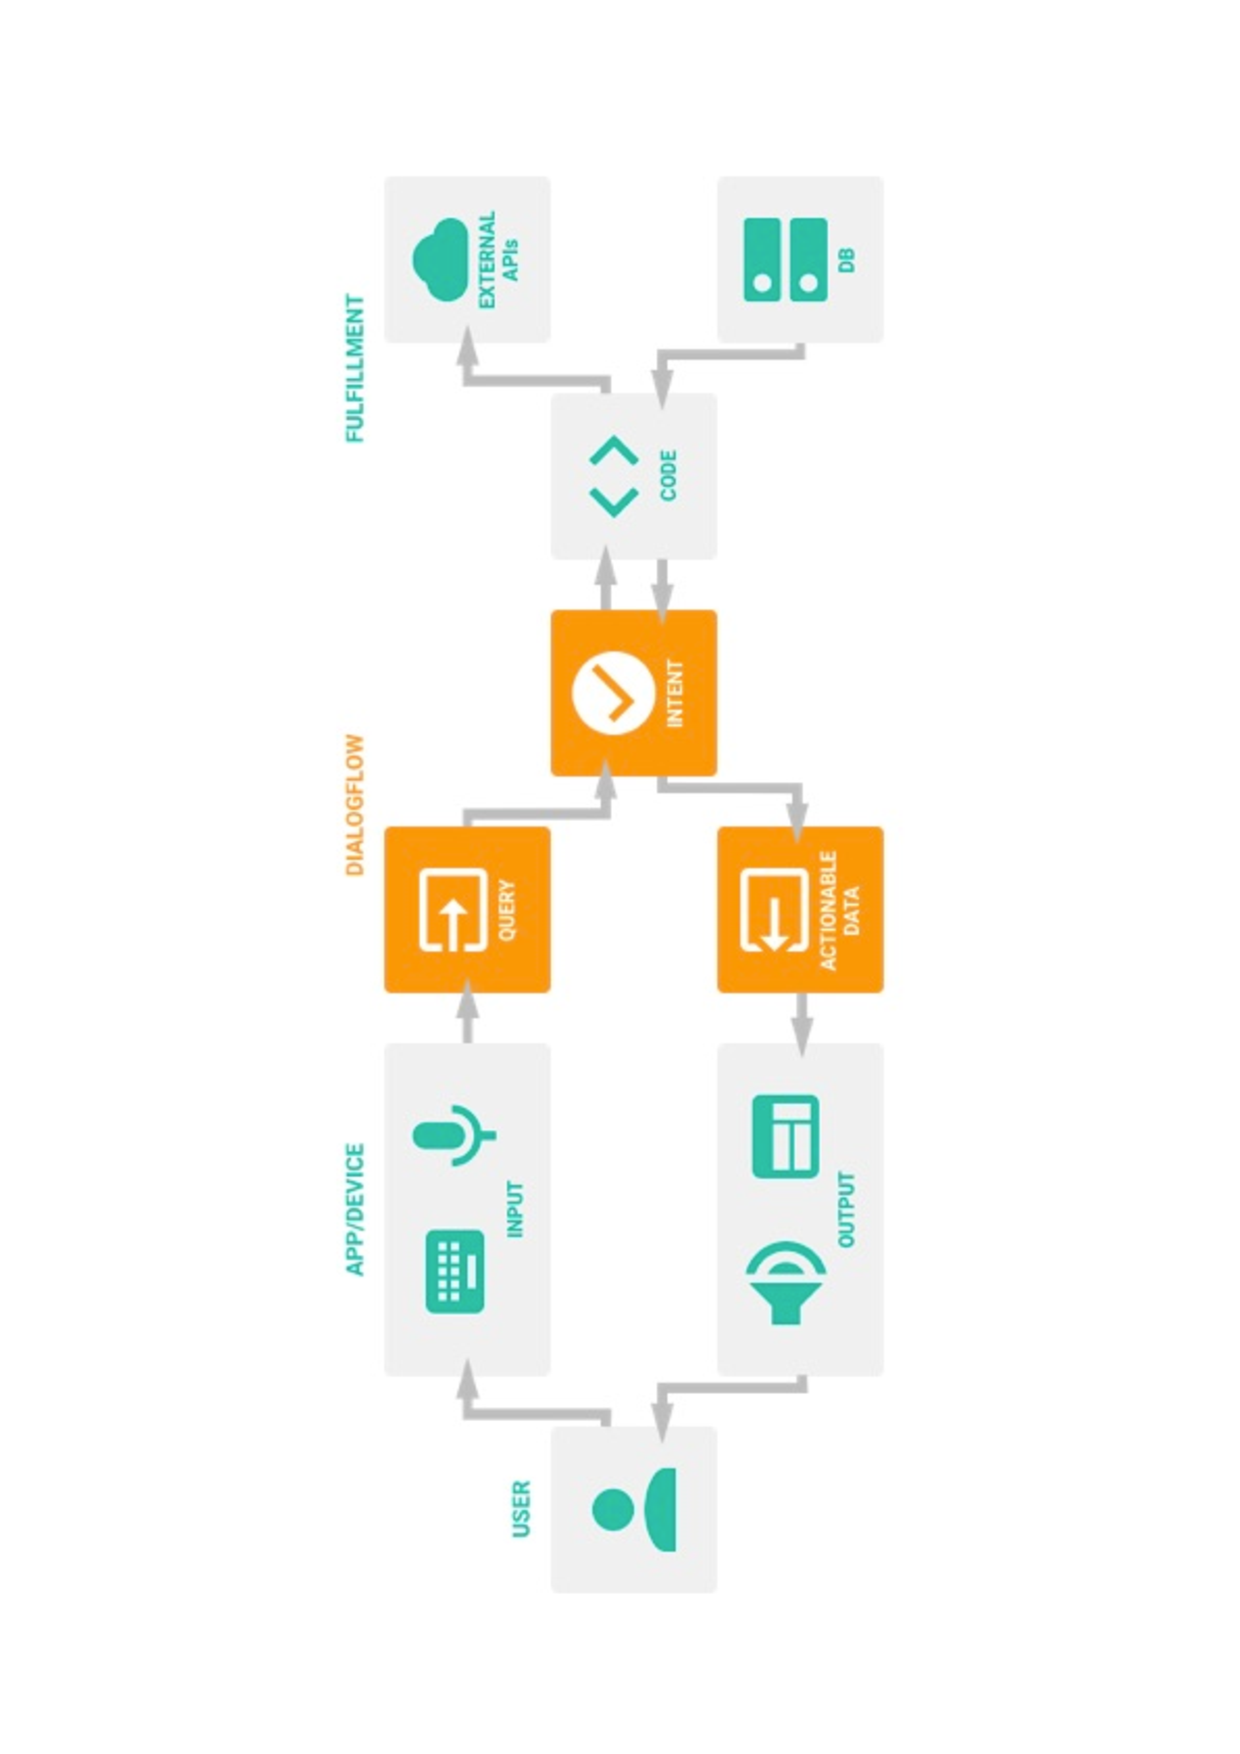
\includegraphics[angle=270,scale=.3]{dialogflowGlossary.pdf}
\end{figure}
\begin{enumerate}
\item agent [ Name of your app ] - 
\par Agents are best described as NLU (Natural Language Understanding) modules. These can be included in your app, product, or service and transform natural user requests into actionable data.
Agent is the name of your app you are creating. The name of the agent is very important. Here is few guidelines while picking the name:
You need to invoke your agent by saying:
“Okay Google, talk to <app name>”

\item intent [ conversation starter ] - 
\par Whenever the user ask a question, it will try to match in corresponding Intent. Intent plays vital role in the assistant app. In Dialogflow, an intent houses elements and logic to parse information from the user and answer their requests.
To understand the question better by intent we (developer) need to feed as much as data we can. The more variations added to the intent, the better the agent will comprehend the user. Developer need to think of different variations of same question.

\item entity [ variables ] - 
\par The Dialogflow agent needs to know what information is useful for answering the user’s request. These pieces of data are called entities. Assume them to be dynamic variables.

\item fulfilment [ Custom code ]
\par Dialogflow backed by Google hence it works on cloud functions. When you need to add some custom code you can do it under the fulfilment tab. Fulfilment is where your custom code goes and bind your intent to cloud functions.

\item context
\par Context plays vital role in the success of assistant. How? Context helps the assistant to talk more like human by maintaing the context and replying in the context to end users.

\item Platform Integration
\par Dialogflow is an open platform as it not only support the integration to Assistant app it support integration to more than 20+ platform such as twitter, Facebook, Slack etc.
\end{enumerate}
\begin{figure}[h]
\centering
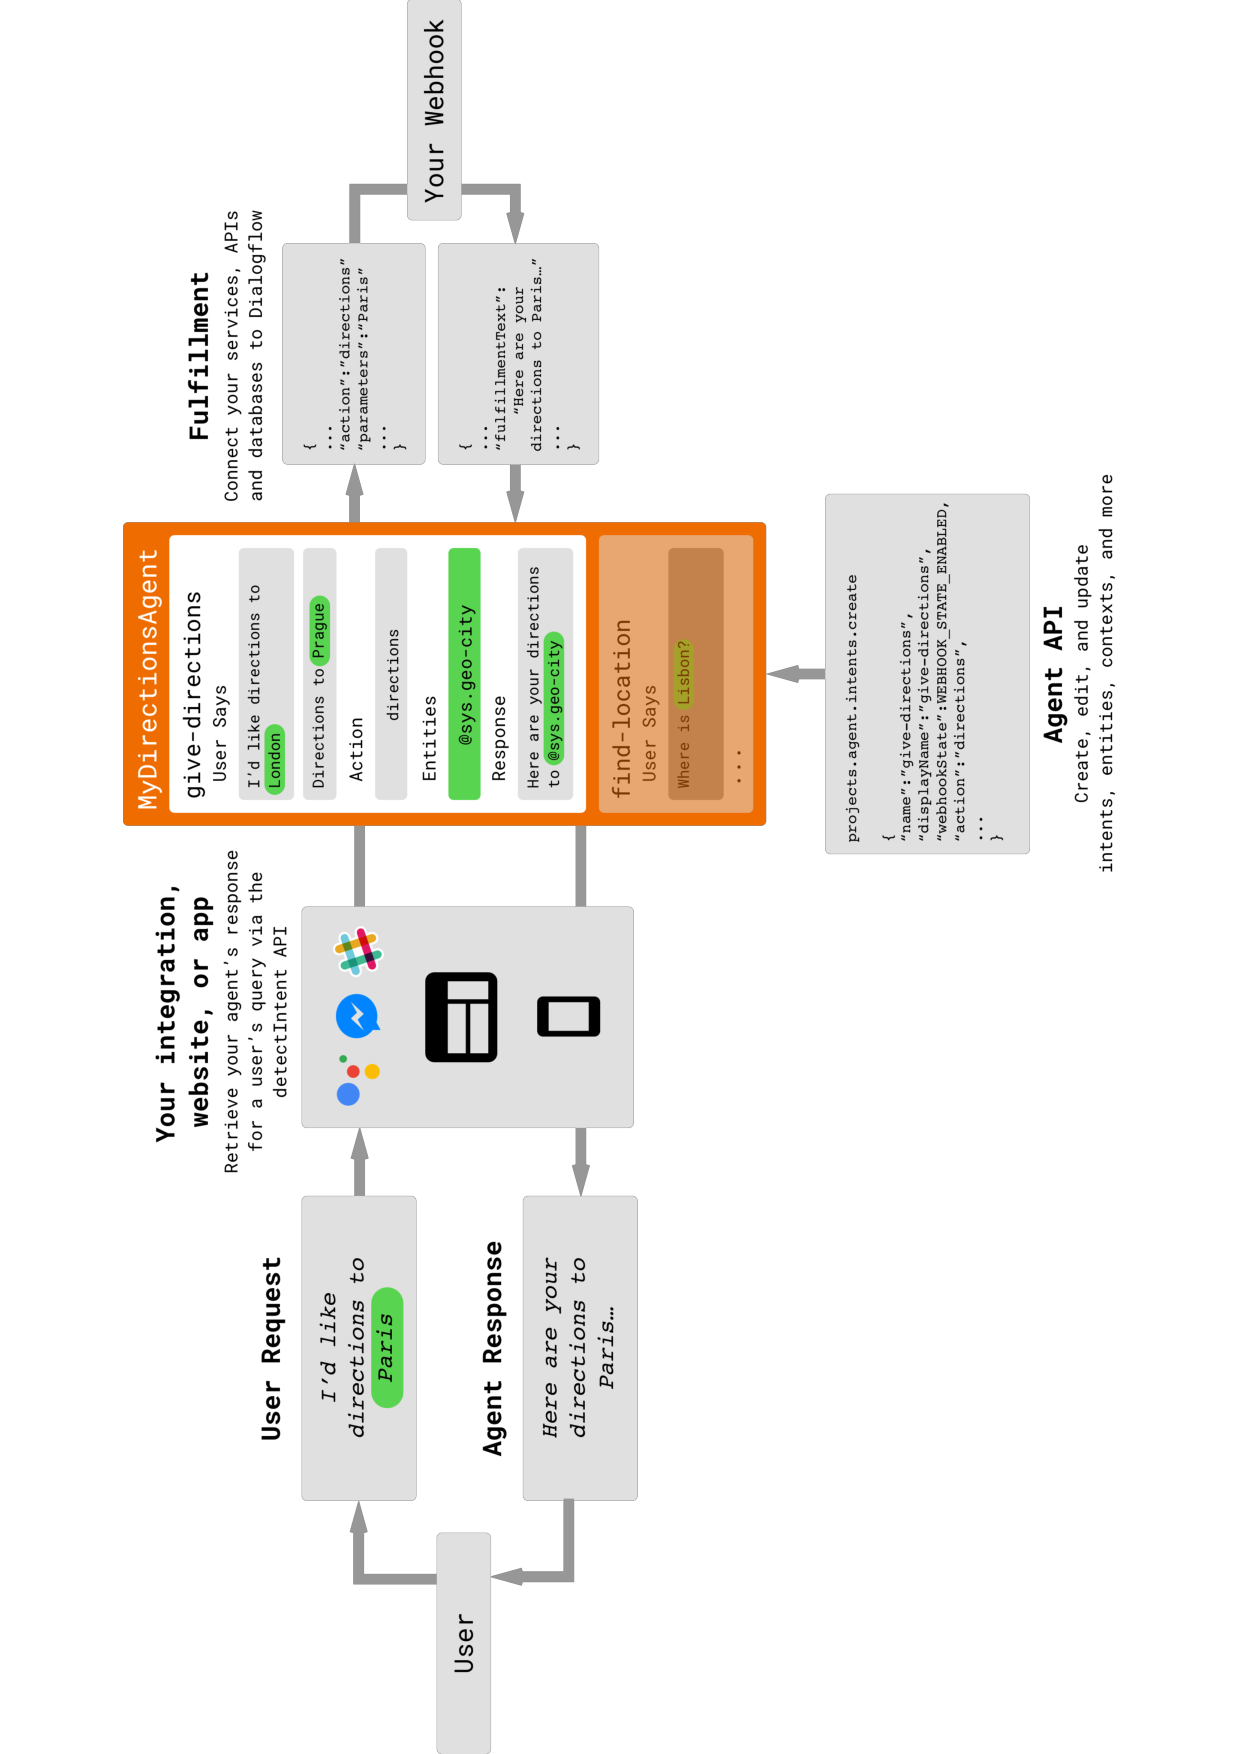
\includegraphics[angle=270,scale=.4]{dialogflowFlow.pdf}
\end{figure}
\newpage
\section{Tensorflow}
\subsection{Introduction to Tensorflow}
\par TensorFlow is an open-source machine learning library for research and production. TensorFlow offers APIs for beginners and experts to develop for desktop, mobile, web, and cloud.TensorFlow is an open-source machine learning library for research and production. TensorFlow offers APIs for beginners and experts to develop for desktop, mobile, web, and cloud.
TensorFlow can run on multiple CPUs and GPUs (with optional CUDA and SYCL extensions for general-purpose computing on graphics processing units). TensorFlow is available on 64-bit Linux, macOS, Windows, and mobile computing platforms including Android and iOS.
Its flexible architecture allows for the easy deployment of computation across a variety of platforms (CPUs, GPUs, TPUs), and from desktops to clusters of servers to mobile and edge devices.
TensorFlow provides stable Python and C APIs; and without API backwards compatibility guarantee: C++, Go, Java, JavaScript and Swift. Third party packages are available for C\#, Haskell, Julia, R, Scala, Rust, OCaml, and Crystal.

\subsection{Use cases of Tensorflow}
\begin{enumerate}
\item Voice/Sound Recognition :
\par One of the most well-known uses of TensorFlow are Sound based applications. With the proper data feed, neural networks are capable of understanding audio signals. These can be :
\begin{itemize}
\item[•] Voice recognition – mostly used in IoT, Automotive, Security and UX/UI.
\item[•] Voice search – mostly used in Telecoms, Handset Manufacturer.
\item[•] Sentiment Analysis – mostly used in CRM.
\item[•] Flaw Detection (engine noise) – mostly used in Automotive and Aviation.
\end{itemize}
\par Regarding common use cases, we are all familiar with voice-search and voice-activated assistants with the new wide spreading smartphones such as Apple’s Siri, Google Now for Android and Microsoft Cortana for Windows Phone.
Language understanding is another common use case for Voice Recognition. Speech-to-text applications can be used to determine snippets of sound in greater audio files, and transcribe the spoken word as text.
Sound based applications also can be used in CRM. A use case scenario might be: TensorFlow algorithms standing in for customer service agents, and route customers to the relevant information they need, and faster than the agents.

\item Text Based Applications :
\par Further popular uses of TensorFlow are, text based applications such as sentimental analysis (CRM, Social Media), Threat Detection (Social Media, Government) and Fraud Detection (Insurance, Finance).
\par Language Detection is one of the most popular uses of text based applications. We all know Google Translate, which supports over 100 languages translating from one to another. The evolved versions can be used for many cases like translating jargon legalese in contracts into plain language.
\par Google also found out that for shorter texts, summarisation can be learned with a technique called sequence-to-sequence learning. This can be used to produce headlines for news articles. Below, you can see an example where the model reads the article text and writes a suitable headline.
\par Another Google use case is SmartReply. It automatically generates e-mail responses (wishing for the evolved version of this one doing our business on behalf of us).

\item Image Recognition :
\par Mostly used by Social Media, Telecom and Handset Manufacturers; Face Recognition, Image Search, Motion Detection, Machine Vision and Photo Clustering can be used also in Automotive, Aviation and Healthcare Industries. Image Recognition aims to recognise and identify people and objects in images as well as understanding the content and context.
\par TensorFlow object recognition algorithms classify and identify arbitrary objects within larger images. This is usually used in engineering applications to identify shapes for modelling purposes (3D space construction from 2D images) and by social networks for photo tagging (Facebook’s Deep Face). By analysing thousands of photos of trees for example, the technology can learn to identify a tree it has never seen before.
\par Image Recognition is starting to expand in the Healthcare Industry, too where TensorFlow algorithms can process more information and spot more patterns than their human counterparts. Computers are now able to review scans and spot more illnesses than humans.

\item Time Series :
\par TensorFlow Time Series algorithms are used for analysing time series data in order to extract meaningful statistics. They allow forecasting non-specific time periods in addition to generate alternative versions of the time series.
\par The most common use case for Time Series is Recommendation. You’ve probably heard of this use from Amazon, Google, Facebook and Netflix where they analyse customer activity and compare it to the millions of other users to determine what the customer might like to purchase or watch.  These recommendations are getting even smarter, for example, they offer you certain things as gifts (not for yourself) or TV shows that your family members might like.
\par The other uses of TensorFlow Time Series algorithms are mainly the field of interest to Finance, Accounting, Government, Security and IoT with Risk Detections, Predictive Analysis and Enterprise/Resource Planning.

\item Video Detection :
\par TensorFlow neural networks also work on video data. This is mainly used in Motion Detection, Real-Time Thread Detection in Gaming, Security, Airports and UX/UI fields.  Recently, Universities are working on Large scale Video Classification datasets like YouTube-8M aiming to accelerate research on large-scale video understanding, representation learning, noisy data modelling, transfer learning, and domain adaptation approaches for video.

\item As TensorFlow is an open source library, we will see many more innovative use cases soon, which will influence one another and contribute to Machine Learning technology.
\end{enumerate}

\newpage
\section{Apple Inc. provided APIs / Libraries}
\subsection{Core ML}
\par With Core ML, you can integrate trained machine learning models into your app.
\par A trained model is the result of applying a machine learning algorithm to a set of training data. The model makes predictions based on new input data. For example, a model that's been trained on a region's historical house prices may be able to predict a house's price when given the number of bedrooms and bathrooms.
\par Core ML is the foundation for domain-specific frameworks and functionality. Core ML supports Vision for image analysis, Natural Language for natural language processing, and GameplayKit for evaluating learned decision trees. Core ML itself builds on top of low-level primitives like Accelerate and BNNS, as well as Metal Performance Shaders.
\par Core ML is optimised for on-device performance, which minimises memory footprint and power consumption. Running strictly on the device ensures the privacy of user data and guarantees that your app remains functional and responsive when a network connection is unavailable.
\begin{figure}[h]
\centering
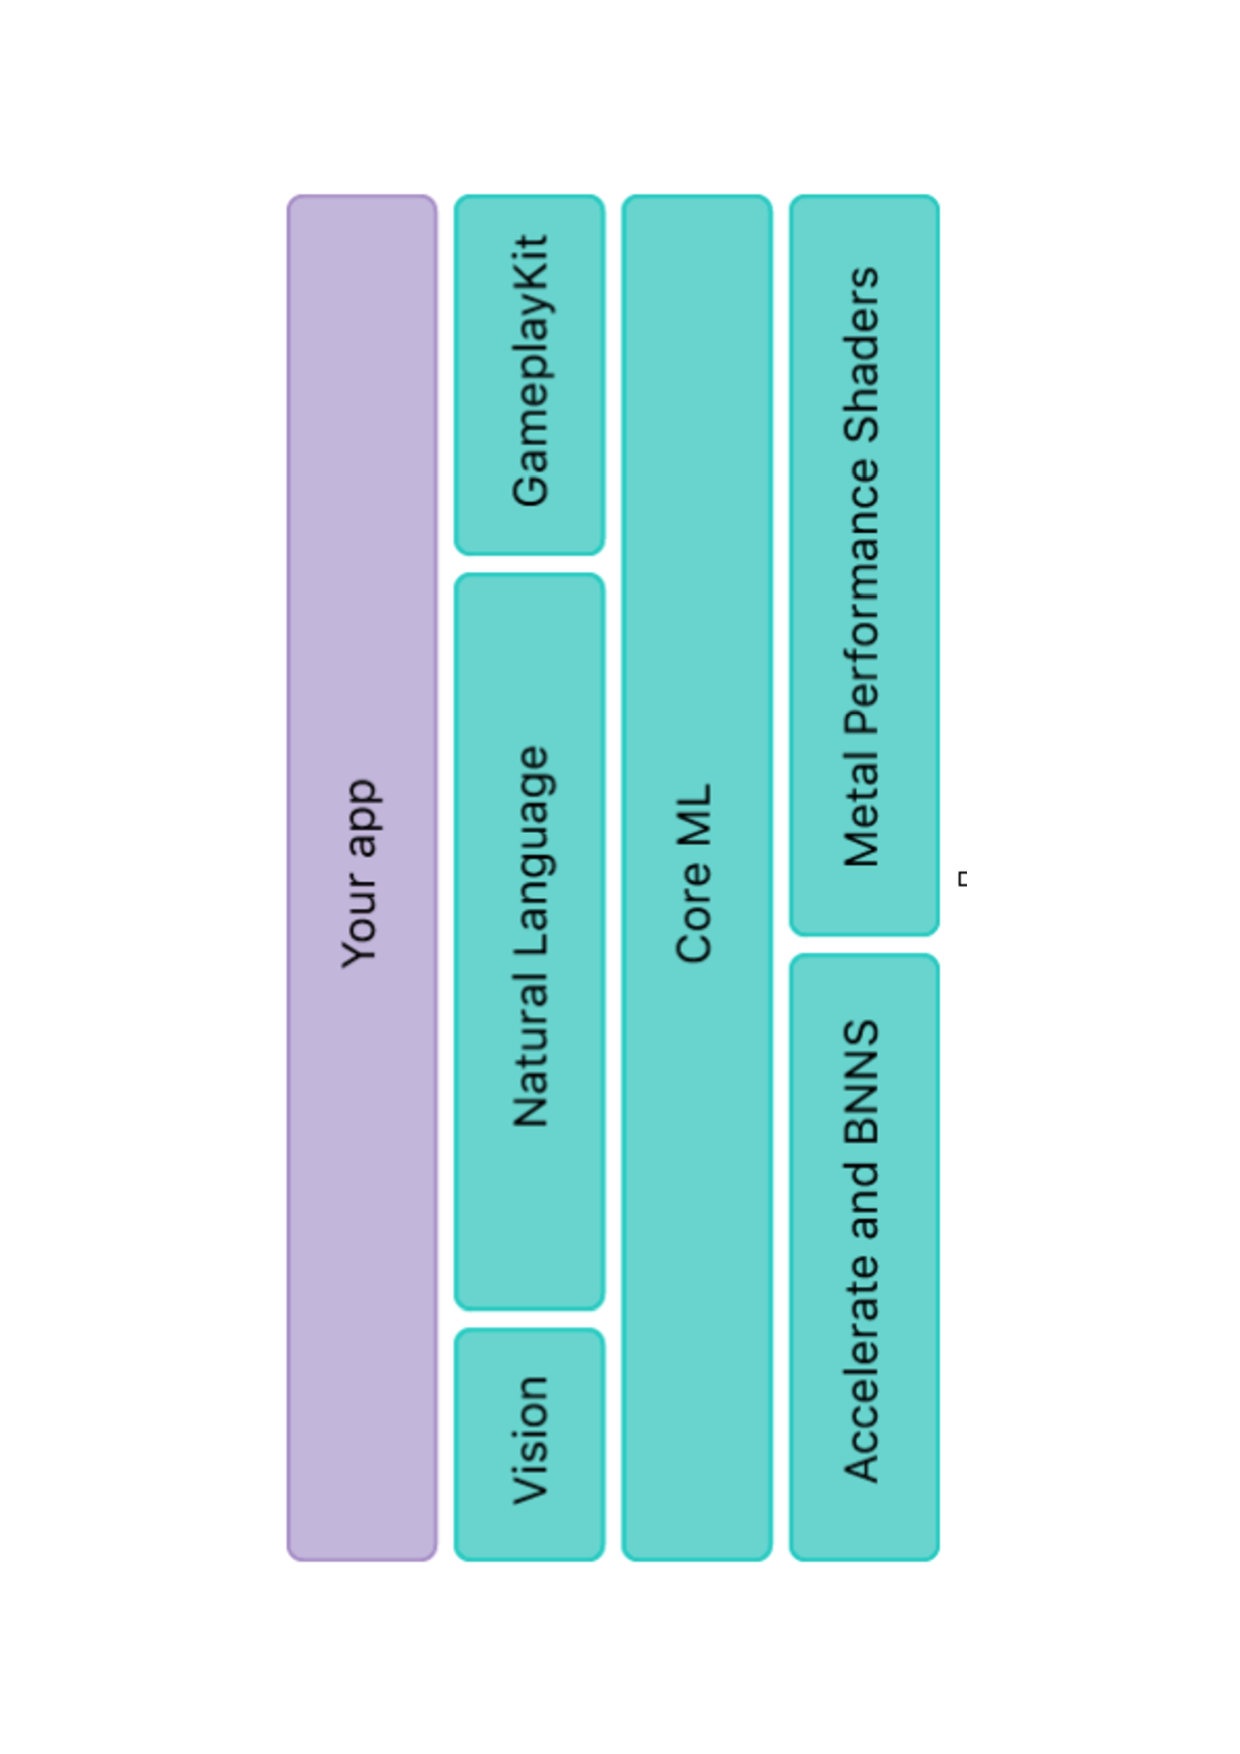
\includegraphics[scale=.5,angle=270]{coreML.pdf}
\end{figure}

\subsection{SiriKit}
\par SiriKit enables your iOS apps and watchOS apps to work with Siri, so users can get things done using just their voice. Your content and services can be used in new scenarios, including access from the lock screen and hands-free use.
\par Siri Suggestions. Using signals like location, time of day and type of motion (such as walking, running or driving), Siri Suggestions learns when to suggest relevant shortcuts.
Notifications. Shortcuts appear as notifications on the lock screen, and users tap the notification to run the task.
\par On-device. All learning is done locally on the device, so Siri creates an intelligent, personalised experience without compromising your privacy.
\par SiriKit encompasses the Intents and Intents UI frameworks, which you use to implement app extensions that integrate your services with Siri. SiriKit supports two types of app extensions :
\begin{enumerate}
\item[•] An Intents app extension receives user requests from SiriKit and turns them into app-specific actions. For example, the user might ask Siri to send a message, book a ride, or start a workout using your app.
\item[•] An Intents UI app extension displays branding or other customised content in the Siri or Maps interface after your Intents app extension fulfils a user request. Creation of this extension is optional.
\end{enumerate}
\par SiriKit defines the types of requests—known as intents—that users can make. Related intents are grouped into domains to make it clear which intents you might support in your app. For example, the messages domain has intents for sending messages, searching for messages, and marking messages as read or unread.
\par Your app extensions rarely communicate with the user directly. Siri and Maps typically handle all communication with the user and call out to your extensions only when they need you to provide information. You can provide an Intents UI app extension to customise the information that Siri and Maps display, but doing so is optional.
\begin{figure}[h]
\centering
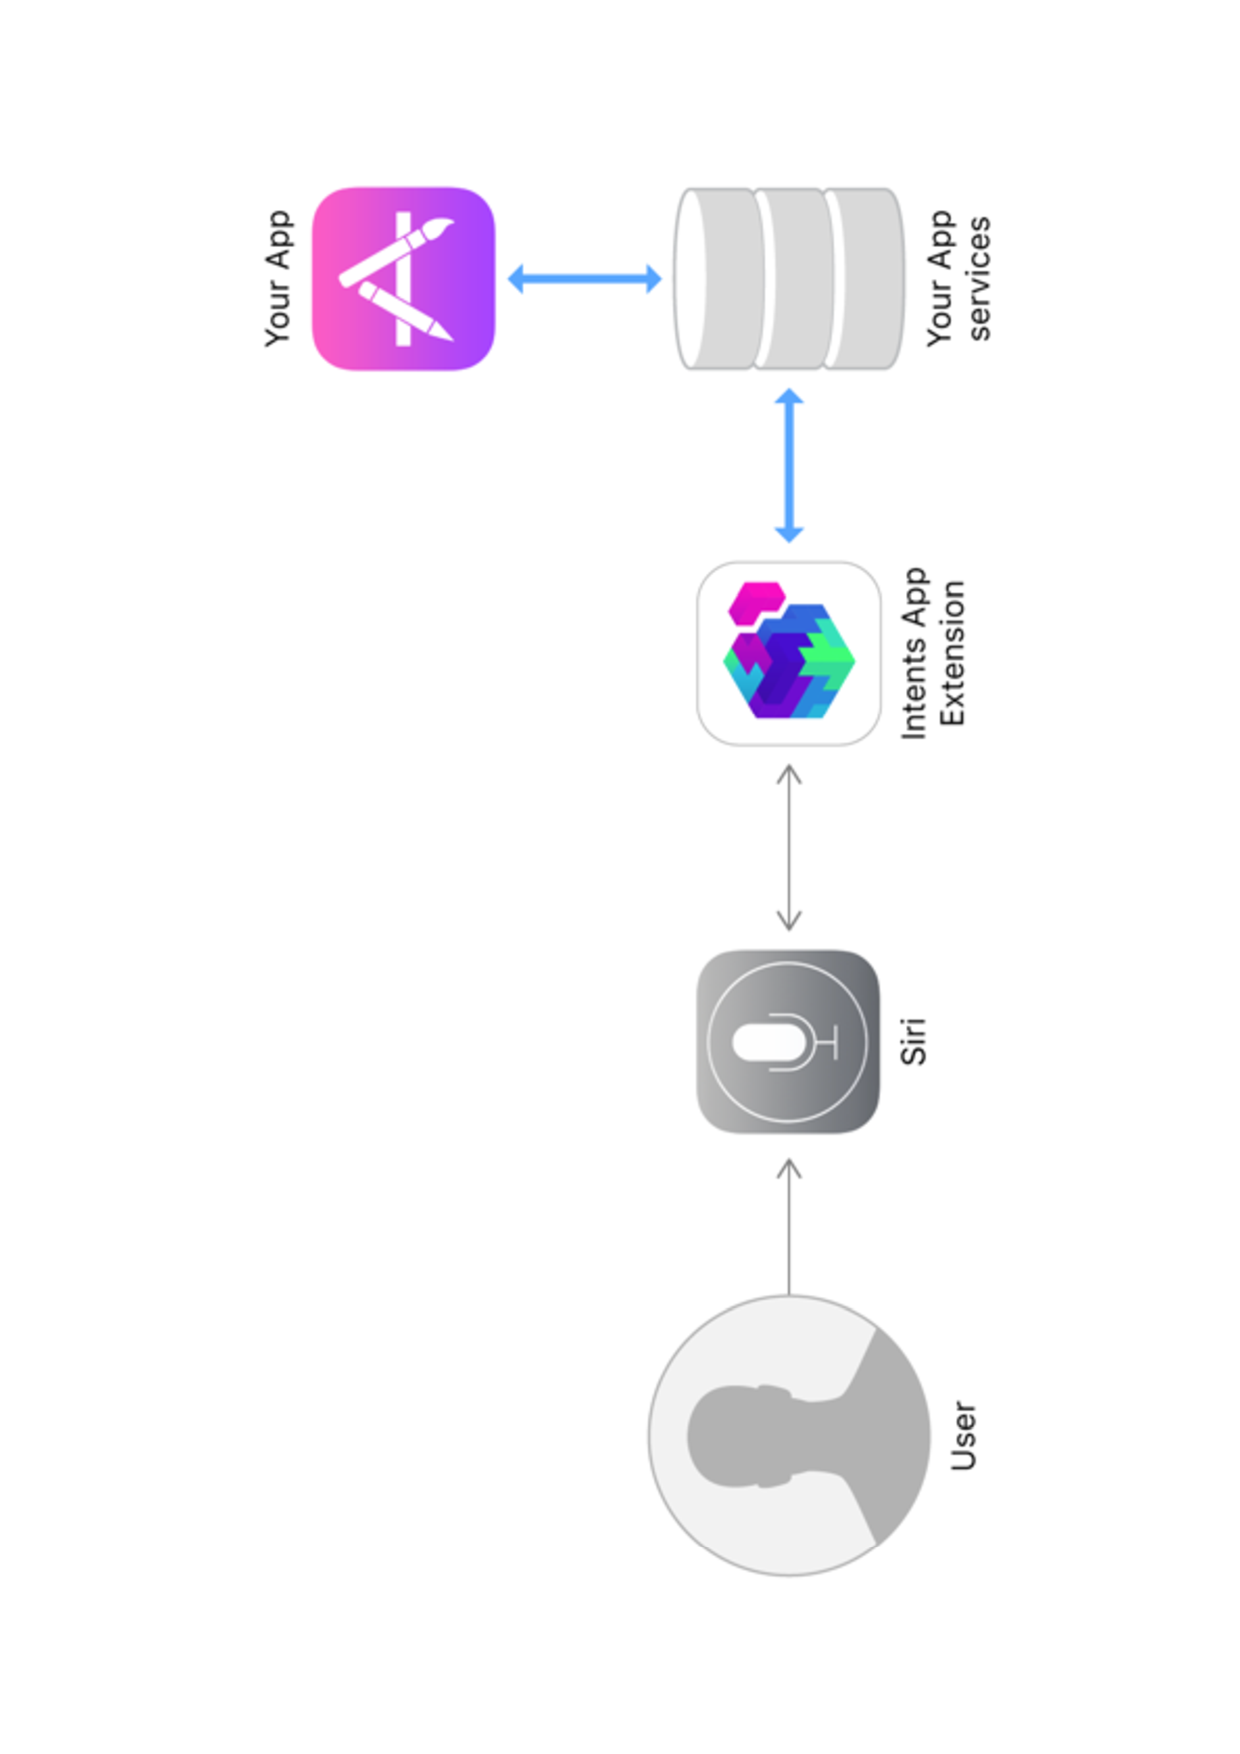
\includegraphics[scale=.5,angle=270]{siriKit.pdf}
\end{figure}
\newpage
\section{Amazon Inc. provided APIs / Libraries}
\subsection{Alexa Voice Service}
\par Amazon allows device manufacturers to integrate Alexa voice capabilities into their own connected products by using the Alexa Voice Service (AVS), a cloud-based service that provides APIs to interface with Alexa. Products built using AVS have access to Alexa's growing list of capabilities including all of the Alexa Skills. AVS provides cloud-based automatic speech recognition (ASR) and natural language understanding (NLU). There are no fees for companies looking to integrate Alexa into their products by using AVS.
\par he voice of Amazon Alexa is generated by a long short-term memory artificial neural network.

\subsection{Alexa Skills Kit}
\par Amazon allows developers to build and publish skills for Alexa using the Alexa Skills Kit known as Alexa Skills. These third-party developed skills, once published, are available across Alexa-enabled devices. Users can enable these skills using the Alexa app.
\par A "Smart Home Skill API" is available, meant to be used by hardware manufacturers to allow users to control smart home devices.
\par Most skills run code almost entirely in the cloud, using Amazon's AWS Lambda service.
In April 2018, Amazon launched Blueprints, a tool for individuals to build skills for their personal use.
\par In February 2019, Amazon further expanded the capability of Blueprints by allowing customers to publish skills they've built with the templates to its Alexa Skill Store in the US for use by anyone with an Alexa-enabled device.

\subsection{Amazon Lex}
\par Amazon Lex is a service for building conversational interfaces into any application using voice and text. It powers the Amazon Alexa virtual assistant. In April 2017, the platform was released to the developer community, and suggested that it could be used for conversational interfaces (chatbots or otherwise) including Web, mobile apps, robots, toys, drones, and more. Amazon already had launched Alexa Voice Services, which developers can use to integrate Alexa into their own devices, like smart speakers, alarm clocks, etc., however Lex will not require that end users interact with the Alexa assistant per se, but rather any type of assistant or interface.

\newpage
\section{Introduction to AI using Python}

\subsection{Computer Vision using OpenCV}
\par OpenCV (Open Source Computer Vision Library) is an open source library of programming functions for computer vision and machine learning software. OpenCV was built to provide a common infrastructure for computer vision applications and to accelerate the use of machine perception in the commercial products.
\par The library has more than 2500 optimised algorithms, which includes a comprehensive set of both classic and state-of-the-art computer vision and machine learning algorithms. These algorithms can be used to detect and recognise faces, identify objects, classify human actions in videos, track camera movements, track moving objects, extract 3D models of objects, produce 3D point clouds from stereo cameras, stitch images together to produce a high resolution image of an entire scene, find similar images from an image database, remove red eyes from images taken using flash, follow eye movements, recognise scenery and establish markers to overlay it with augmented reality, etc. OpenCV has more than 47 thousand people of user community and estimated number of downloads exceeding 14 million. The library is used extensively in companies, research groups and by governmental bodies.The library is cross-platform and free for use under the open-source BSD license.
\par OpenCV supports the deep learning frameworks TensorFlow.

\subsubsection{Python program for Edge Detection}
\par \textbf{CODE}
\begin{lstlisting}
import cv2
import sys

# To Read the image
image = cv2.imread("cards.jpg")

#To convert to grayscale
gray_image = cv2.cvtColor(image, cv2.COLOR_BGR2GRAY)

#To blur the image
blurred_image = cv2.GaussianBlur(gray_image, (7,7), 0)

# Show both our images
cv2.imshow("Original image", image)
cv2.imshow("Blurred image", blurred_image)

# Run the Canny edge detector
canny = cv2.Canny(blurred_image, 30, 100)
cv2.imshow("Canny", canny)

#Finding contours
im, contours, hierarchy= cv2.findContours(canny, cv2.RETR_EXTERNAL, cv2.CHAIN_APPROX_SIMPLE)

print("Number of objects found = ", len(contours))

#Highlighing the contours
cv2.drawContours(image, contours, -1, (0,255,0), 2)
cv2.imshow("objects Found", image)
cv2.waitKey(0)
\end{lstlisting}
\par \textbf{RESULT}
\begin{figure}[h]
\centering
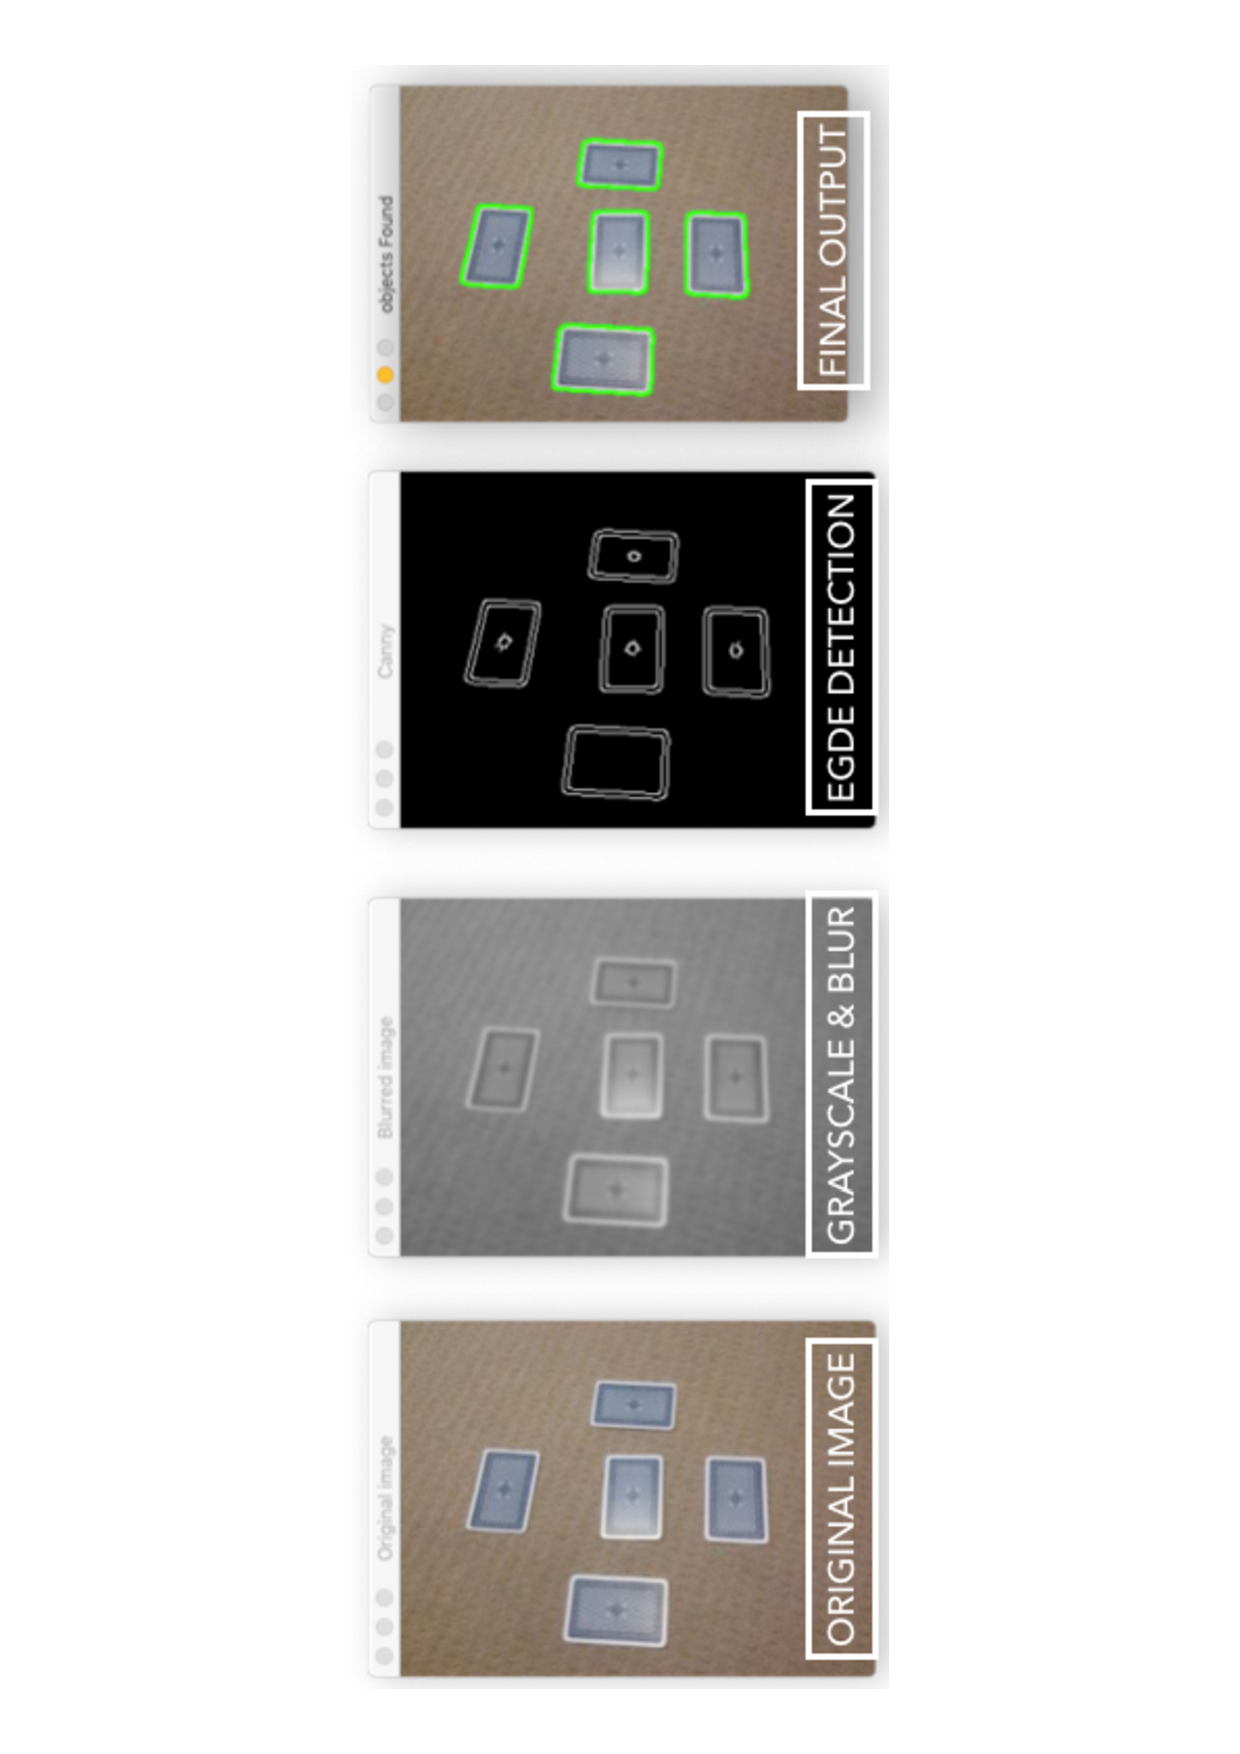
\includegraphics[scale=0.5,angle=270]{pythonED.pdf}
\end{figure}

\par Two important functions in image processing are blurring and grayscale. Many image processing operations take place on grayscale images, as they are simpler to process as they have just two colours. We then detect the contours on the image and highlight to distinguish between objects.
\par The following functions are used to achieve the above output : 
\begin{enumerate}
\item[•] Greyscale - 
\par The function that converts an image to greyscale is cvtColor(). The first argument is the image to be converted, the second is the colour mode. COLOR\_BGR2GRAY stands  for Blue Green Red to Grey.
OpenCV uses the reverse of RGB colour scheme, that is it uses the BGR colour scheme in its parameters.
\item[•] Blur - 
\par The Gaussian blur is the most popular function to blur images, as it offers good blurring at fairly fast speed. The function is GaussinBlur().
\par The first argument is the image itself.
\par The second argument is the window size. Gaussian Blur works over a small window, and blurs all the pixels in that window (by averaging their values). The larger the window, the more blurring will be done, but the code will also be slower. So in the above example we chose a window of (7,7) pixels, which is a box 7 pixels long and 7 pixels wide.
\item[•] Edge Detection - 
\par The function for Canny edge detection is Canny(). It takes three  arguments.
\par The first is the image.
\par The second and third are the lower and upper thresholds respectively.
\par The Canny edge detector detects edges by looking in the difference of pixel intensities.
\par So for the example above, I’m using low thresholds of 30, 100, which means a lot of thresholds will be detected.
\item[•] Find Contours - 
\par The findContours() finds the contours in the given image. The first option is the output of the canny edge detector. RETR\_EXTERNAL tells OpenCv to only find the outermost edges (as you can find contours within contours). The second arguments tells OpenCv to use the simple approximation.
\par The function returns three values: The image, a list of contours found, and the hierarchy (which can be ignored as it is used if you have many contours embedded within others).
\par The contours return value is a simple list that contains the number of contours found. Taking the length of it will give us number of objects found.
\item[•] Draw Contours - 
\par Finally, we use the drawContours() function. The first argument is the image we want to draw on. The second is the contours we found in the last function. The 3rd is -1, to say that we want all contours to be drawn (we can choose to only draw certain contours). The fourth is the colour, green in this case, and the last is the thickness.
\end{enumerate}

\subsubsection{Python program for Face Detection}
\par OpenCV uses machine learning algorithms to search for faces within a picture. For something as complicated as a face, there isn’t one simple test that will tell us if it found a face or not. Instead, there are thousands of small patterns/features that must be matched. The algorithms break the task of identifying the face into thousands of smaller, bite-sized tasks, each of which is easy to solve. These tasks are also called classifiers.
\par For something like a face, we may have 6,000 or more classifiers, all of which must match for a face to be detected (within error limits, of course). But therein lies the problem: For face detection, the algorithm starts at the top left of a picture and moves down across small blocks of data, looking at each block, constantly asking, “Is this a face? … Is this a face? … Is this a face?” Since there are 6,000 or more tests per block, we might have millions of calculations to do, which will grind our computer to a halt.
\begin{figure}[h]
\centering
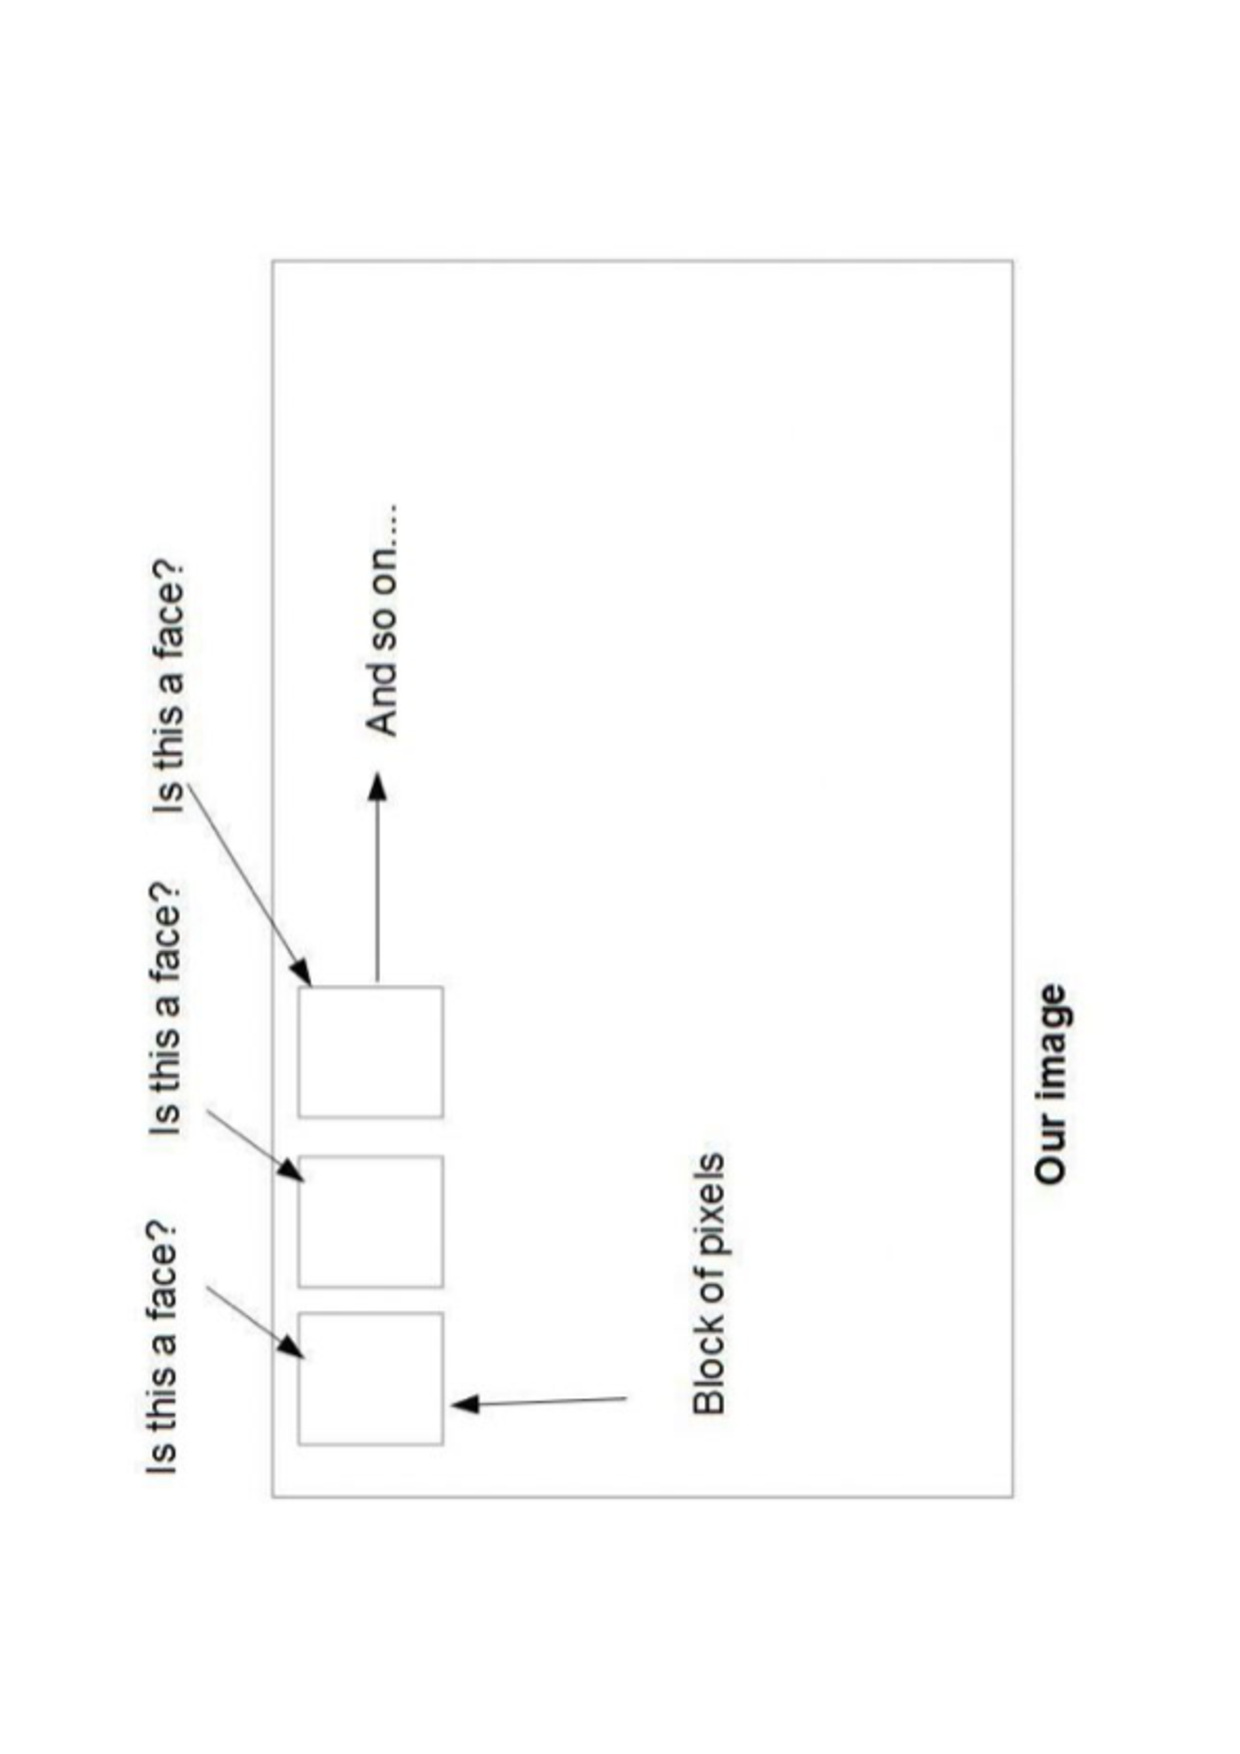
\includegraphics[scale=0.3,angle=270]{pythonFDExample.pdf}
\end{figure}
\par To get around this, OpenCV uses cascades. What’s a cascade? The best answer can be found from the dictionary: A waterfall or series of waterfalls.
\par Like a series of waterfalls, the OpenCV cascade breaks the problem of detecting faces into multiple stages. For each block, it does a very rough and quick test. If that passes, it does a slightly more detailed test, and so on.
\par Since face detection is such a common case, OpenCV comes with a number of built-in cascades for detecting everything from faces to eyes to hands and legs.
\par
\textbf{CODE}
\begin{lstlisting}
import sys
import cv2


imgpath = sys.argv[1]
cascasdepath = "haarcascade_frontalface_default.xml"

image = cv2.imread(imgpath)
#image = cv2.imread('abba.png')
gray = cv2.cvtColor(image, cv2.COLOR_BGR2GRAY)

face_cascade = cv2.CascadeClassifier(cascasdepath)

faces = face_cascade.detectMultiScale(
    gray,
    scaleFactor = 1.2,
    minNeighbors = 5,
    minSize = (30,30)

    )

print("The number of faces found = ", len(faces))

for (x,y,w,h) in faces:
    cv2.rectangle(image, (x,y), (x+h, y+h), (0, 255, 0), 2)

cv2.imshow("Faces found", image)    
cv2.waitKey(0)
\end{lstlisting}
\par \textbf{RESULT}
\begin{figure}[h]
\centering
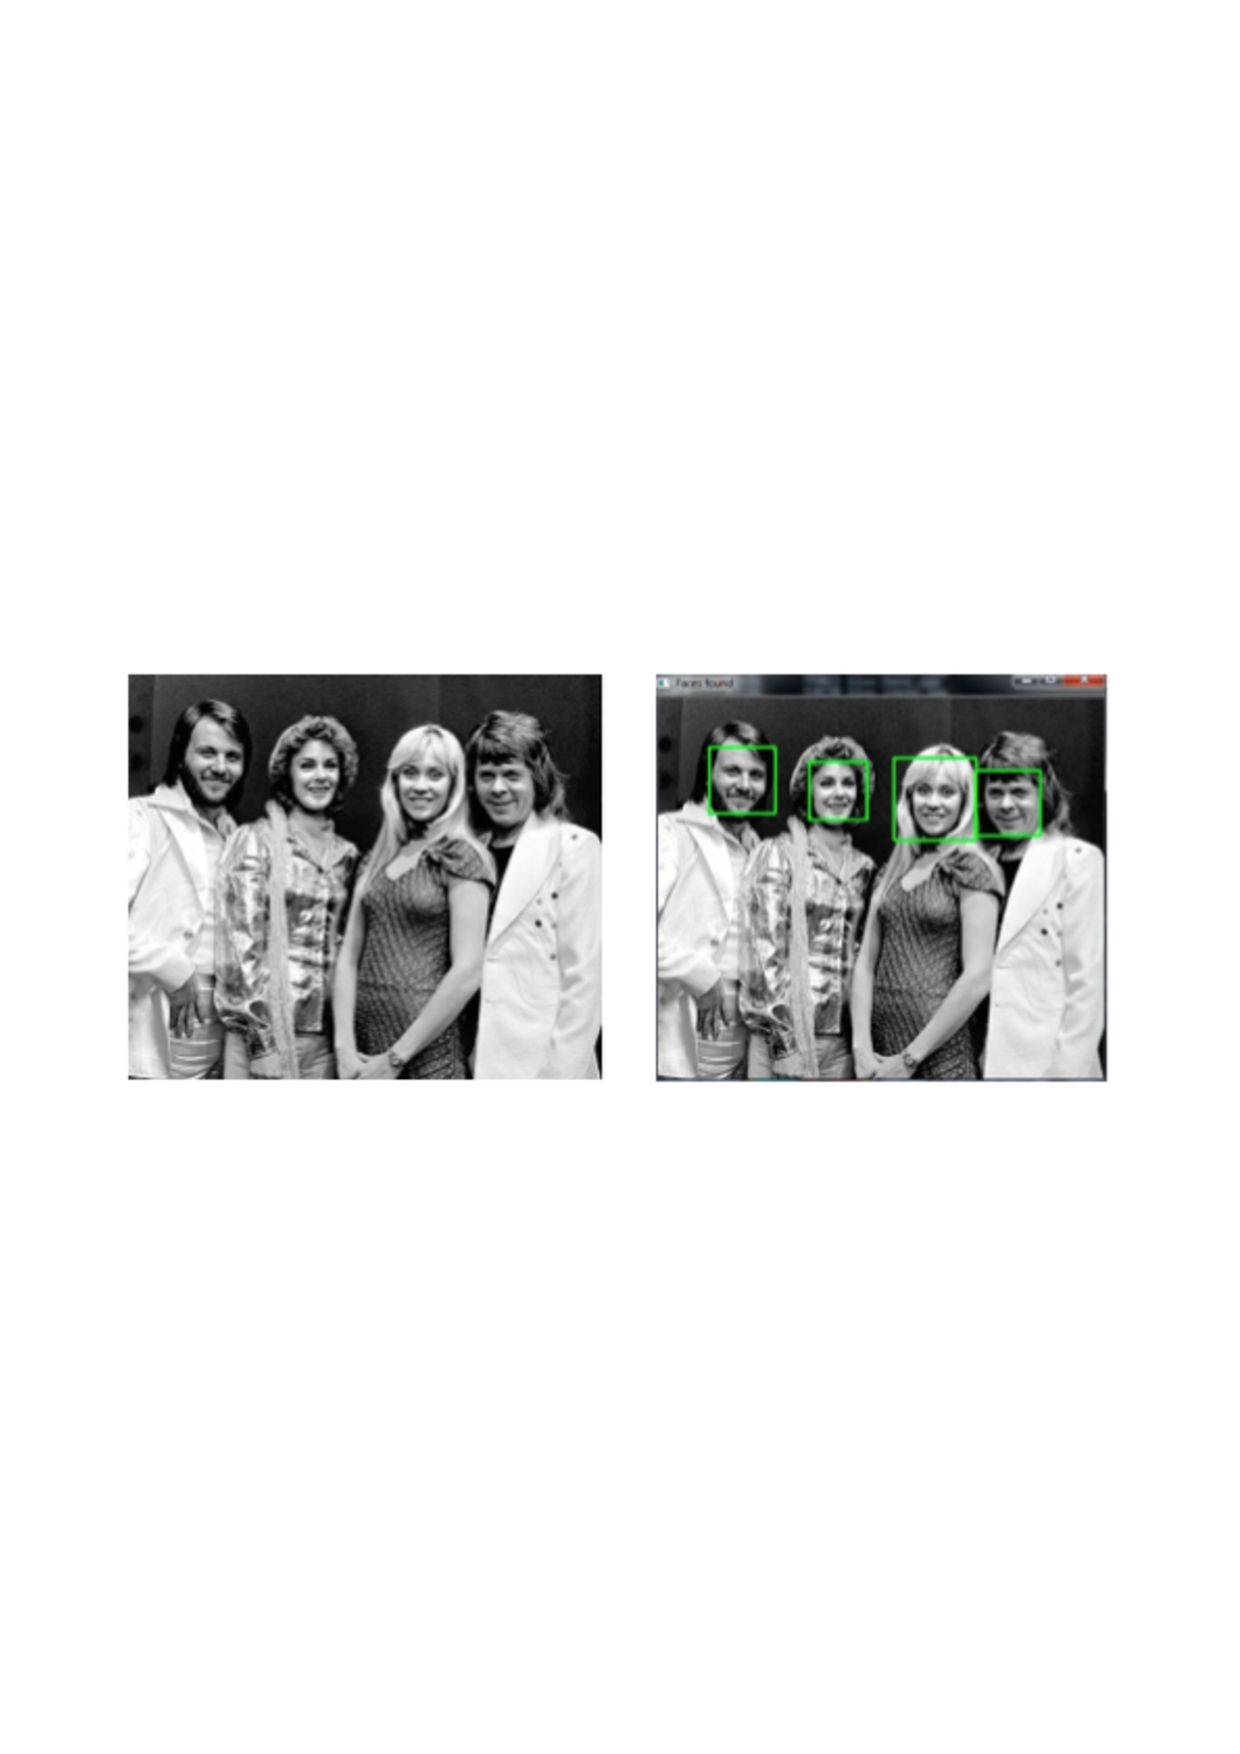
\includegraphics[scale=0.7,angle=0]{pythonFDResult.pdf}
\end{figure}
\par The detectMultiScale() function is a general function that detects objects. Since it is called on the face cascade, that’s what it detects. Its parameters are : 
\begin{enumerate}
\item[•] The first parameter is the grayscale image.
\item[•] The second is the scaleFactor. Since some faces may be closer to the camera, they would appear bigger than those faces in the back. The scale factor compensates for this.
\item[•] The detection algorithm uses a moving window to detect objects. minNeighbors defines how many objects are detected near the current one before it declares the face found. minSize, meanwhile, gives the size of each window.
\end{enumerate}
The function returns a list of rectangles where it believes it found a face.
\newpage
\subsection{Audio and Digital Signal Processing}
\par 
\textbf{CODE}
\begin{lstlisting}
import numpy as np
import wave
import struct
import matplotlib.pyplot as plt

frame_rate = 48000.0
infile = "test.wav"
num_samples = 48000

wav_file = wave.open(infile, 'r')
data = wav_file.readframes(num_samples)
wav_file.close()

data = struct.unpack('{n}h'.format(n=num_samples), data)
data = np.array(data)

data_fft = np.fft.fft(data)

# This will give us the frequency we want
frequencies = np.abs(data_fft)
print("The frequency is {} Hz".format(np.argmax(frequencies)))

plt.subplot(2,1,1)
plt.plot(data[:300])
plt.title("Original audio wave")
plt.subplot(2,1,2)
plt.plot(frequencies)
plt.title("Frequencies found")

plt.xlim(0,1200)
plt.savefig('wave.png').

plt.show()
\end{lstlisting}
\par \textbf{RESULT}
\begin{figure}[h]
\centering
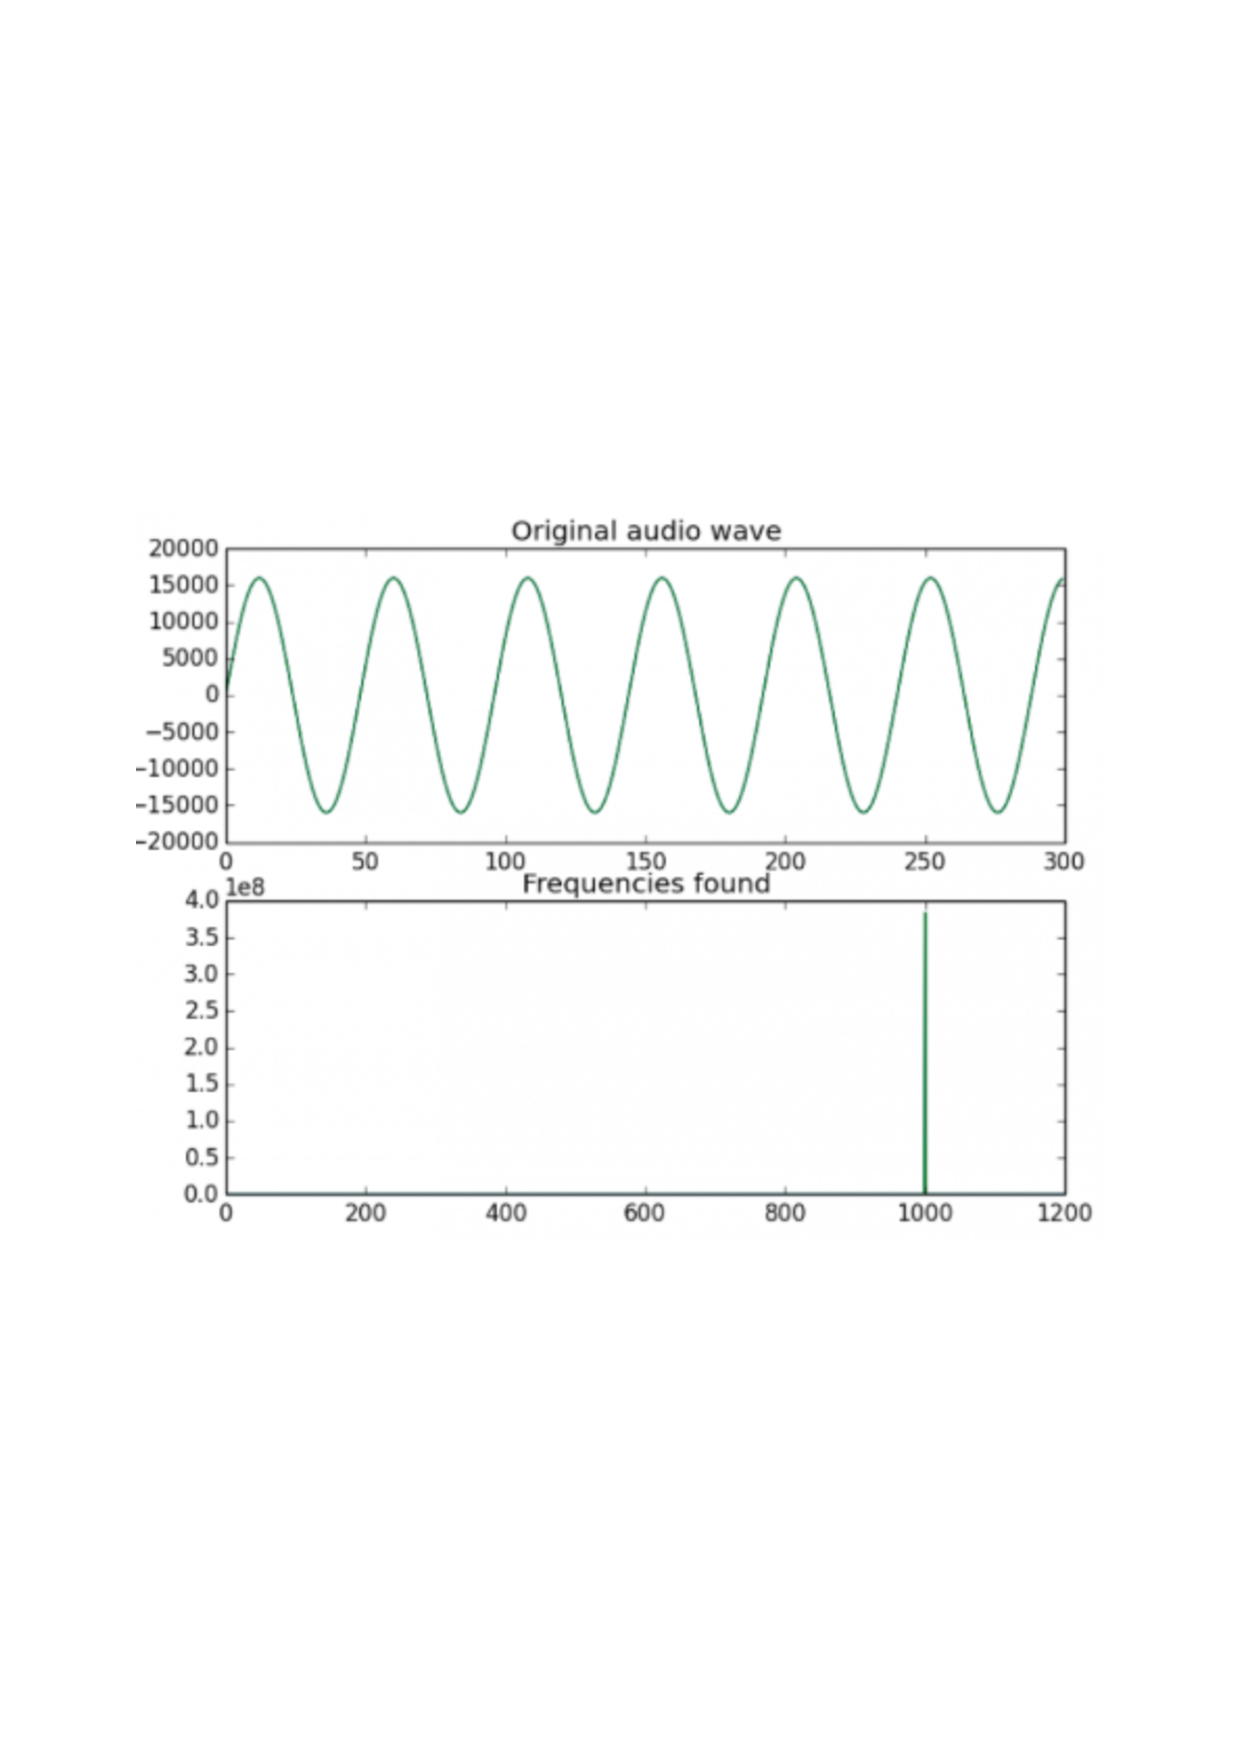
\includegraphics[scale=0.6,angle=0]{pythonDSP.pdf}
\end{figure}
\par To get the frequency of a sine wave, we need to get its Discrete Fourier Transform(DFT).
In its simplest terms, the DFT takes a signal and calculates which frequencies are present in it. In more technical terms, the DFT converts a time domain signal to a frequency domain. For example, let’s look at our sine wave.
The wave is changing with time. If this was an audio file, we could imagine the player moving right as the file plays.
In the frequency domain, we see the frequency part of the signal.The signal will change if we add or remove frequencies, but will not change in time. For example, if we take a 1000 Hz audio tone and take its frequency, the frequency will remain the same no matter how long you look at it. But if you look at it in the time domain, we will see the signal moving.
\par The DFT was really slow to run on computers, so the Fast Fourier Transform (FFT) was invented. The FFT is what is normally used nowadays.
\par Here, we are reading a sample wave file. The wave readframes() function reads all the audio frames from a wave file.
\par We take the fft of the data. This will create an array with all the frequencies present in the signal.
\par np.argmax will return the highest frequency in our signal, which it will then print. As we have seen manually, this is at a $1000Hz$ (or the value stored at data\_fft[1000]). And now we can plot the data too.
\par The function subplot(2,1,1) means that we are plotting a 2x1 grid. The 3rd number is the plot number, and the only one that will change.

\subsection{Natural Language Processing using NLTK}
\subsubsection{Python program using NLTK}
\par NLTK is a leading platform for building Python programs to work with human language data. It provides easy-to-use interfaces to over 50 corpora and lexical resources such as WordNet, along with a suite of text processing libraries for classification, tokenization, stemming, tagging, parsing, and semantic reasoning with wrappers for industrial-strength NLP libraries.
\par PunktSentenceTokenizer is an sentence boundary detection algorithm that must be trained to be used. NLTK already includes a pre-trained version of the PunktSentenceTokenizer. 
\par This tokenizer divides a text into a list of sentences by using an unsupervised algorithm to build a model for abbreviation words, collocations, and words that start sentences.  It must be trained on a large collection of plaintext in the target language before it can be used.
\par This approach has been shown to work well for many European languages.
\par 
\textbf{CODE}
\begin{lstlisting}
#Using the nltk library for natural language processing in python
import nltk

from nltk.tokenize import PunktSentenceTokenizer
 
#Sample sentence
document = 'Whether you\'re new to programming or an experienced developer, it\'s easy to learn and use Python.'

sentences = nltk.sent_tokenize(document)   
for sent in sentences:
    print(nltk.pos_tag(nltk.word_tokenize(sent)))
\end{lstlisting}
\par \textbf{RESULT}
\begin{figure}[h]
\centering
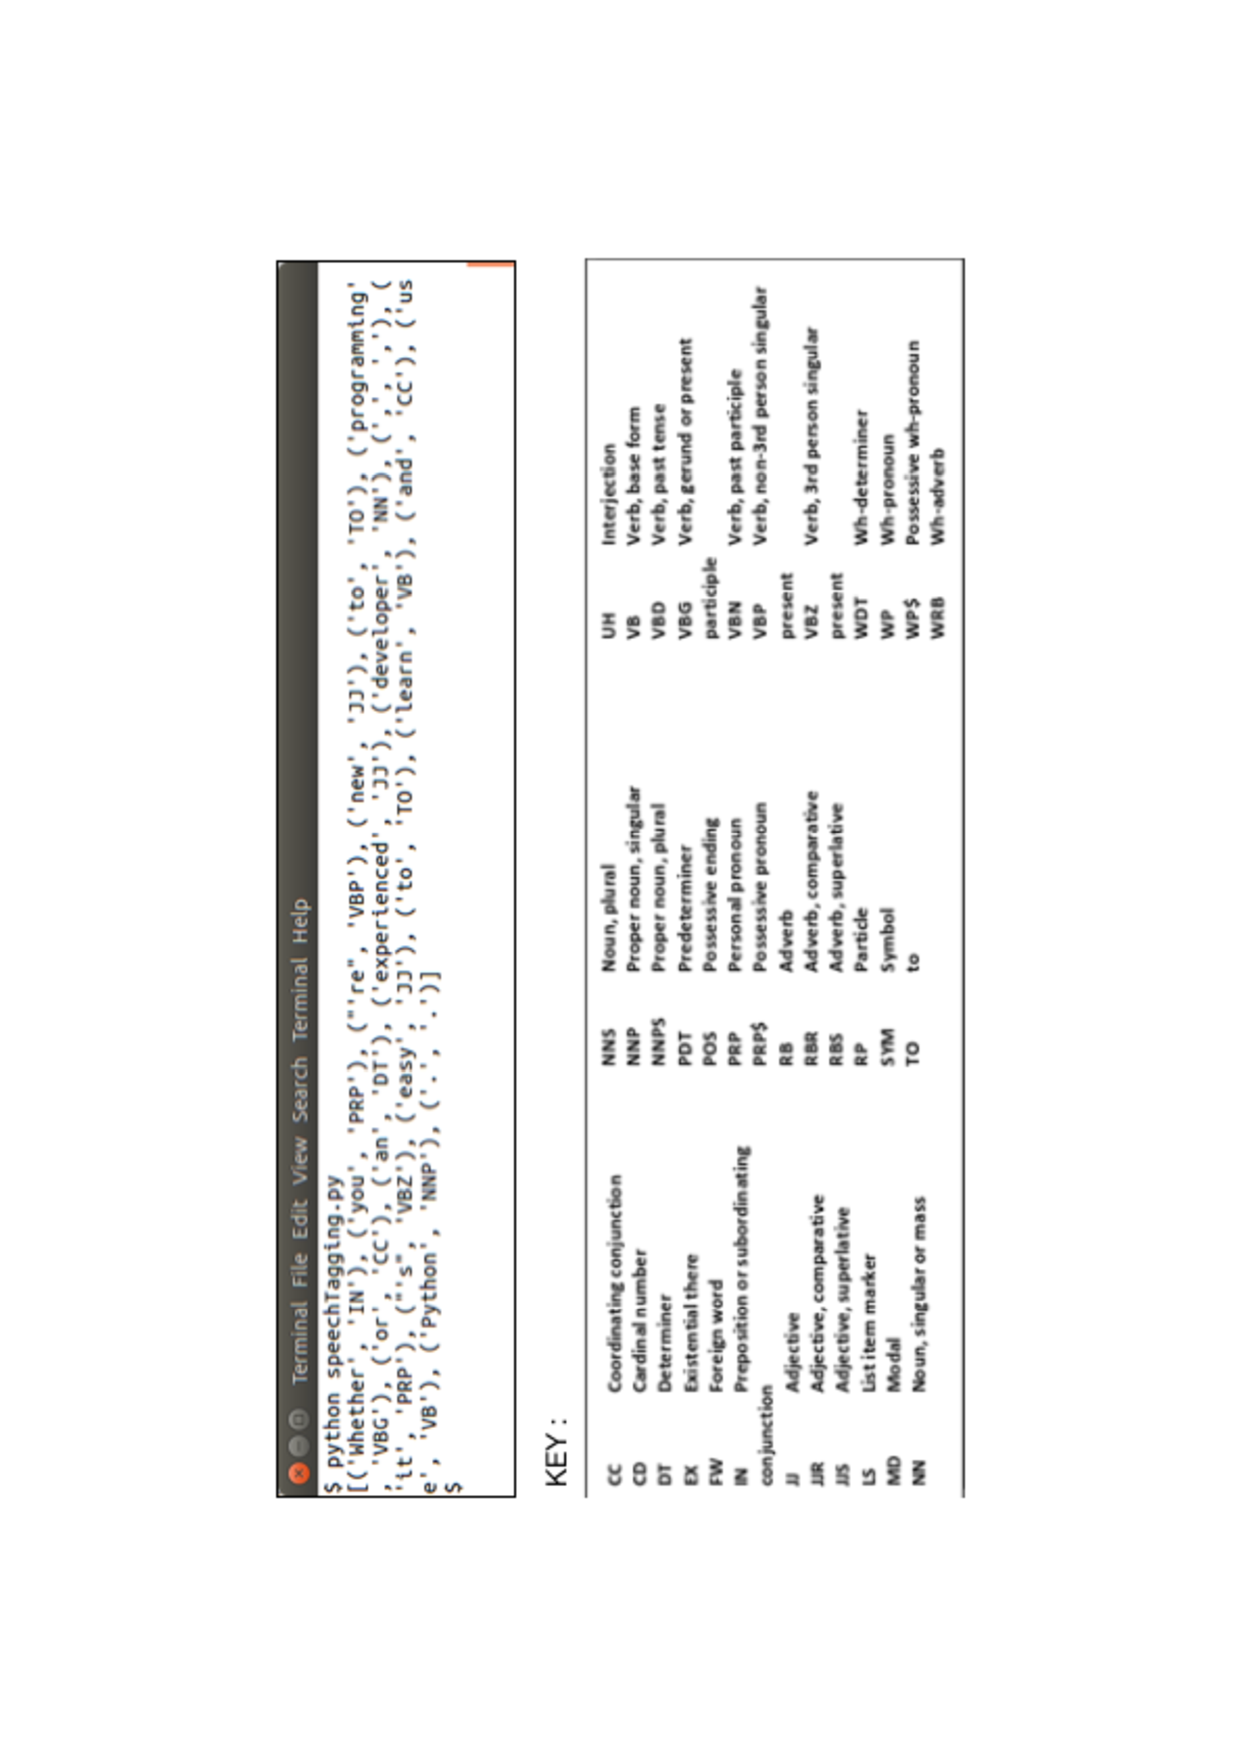
\includegraphics[scale=0.7,angle=270]{pythonNLP.pdf}
\end{figure}
\newpage
\section{References}
\begin{enumerate}
\item https://dialogflow.com/docs/
\item https://www.tensorflow.org/tutorials/
\item https://developer.apple.com/documentation/coreml/
\item https://developer.apple.com/documentation/sirikit 
\item https://developer.amazon.com/alexa-skills-kit/
\item https://developer.amazon.com/alexa-voice-service/
\item https://docs.aws.amazon.com/lex/index.html/
\item https://www.makeuseof.com/tag/diy-google-home-assistant-raspberry-pi/
\item https://www.nltk.org
\item https://www.pythonforengineers.com/articles/
\end{enumerate}
\end{document}
